\documentclass{standalone}
\usepackage{tikz}
\usetikzlibrary{patterns,decorations.pathmorphing}
\begin{document}
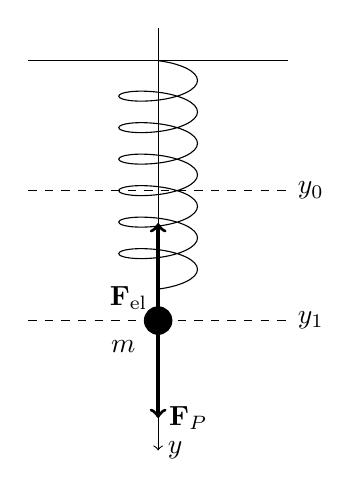
\begin{tikzpicture}[scale=1.65]
    \draw[-](-1,0)--(1,0);
    \draw[->](0,0.25)coordinate(O)--(0,-3)node[right]{$y$};

    \draw[dashed](-1,-1)--(1,-1)node[right]{$y_0$};
    \draw[dashed](-1,-2)--(1,-2)node[right]{$y_1$};


    \draw[decoration={aspect=0.3, segment length=4mm, amplitude=5mm,coil},decorate] (0,0) -- (0,-2); 
    \filldraw[black](0,-2)circle(3pt);
    \node[left]at(-0.1,-2.2){$m$};
    \draw[->,very thick](0,-2)--(0,-2.75)node[right]{$\mathbf{F}_P$};
    \draw[->,very thick](0,-2)node[above left]{$\mathbf{F}_{\mathrm{el}}$}--(0,-1.25);
\end{tikzpicture}
\end{document}